\chapter{Étude d'une trajectoire sur att48}
\section{Ce que compare la figure avant-après}
L'exemple individuel utilise les 48 points d'\code{att48}, exactement dix
stations, $\alpha=1$, la graine 0 et 100 itérations tabou. Chaque itération
évalue 15 candidats et la durée tabou vaut 10. L'exécution dispose donc de
1\,500 évaluations de voisinage. Elle est distincte des trois graines de la
campagne, même si ses paramètres sont identiques à ceux de la graine 0.

La figure~\ref{fig:avantapres} compare la construction initiale à la meilleure
solution trouvée durant cette recherche. Les coordonnées, le nombre de
stations et le poids sont conservés. Ce sont la sélection des stations,
les affectations et l'ordre du cycle qui peuvent changer. La figure ne
représente ni un déplacement des points ni une comparaison entre deux tailles
de réseau.

\begin{figure}[htbp]\centering
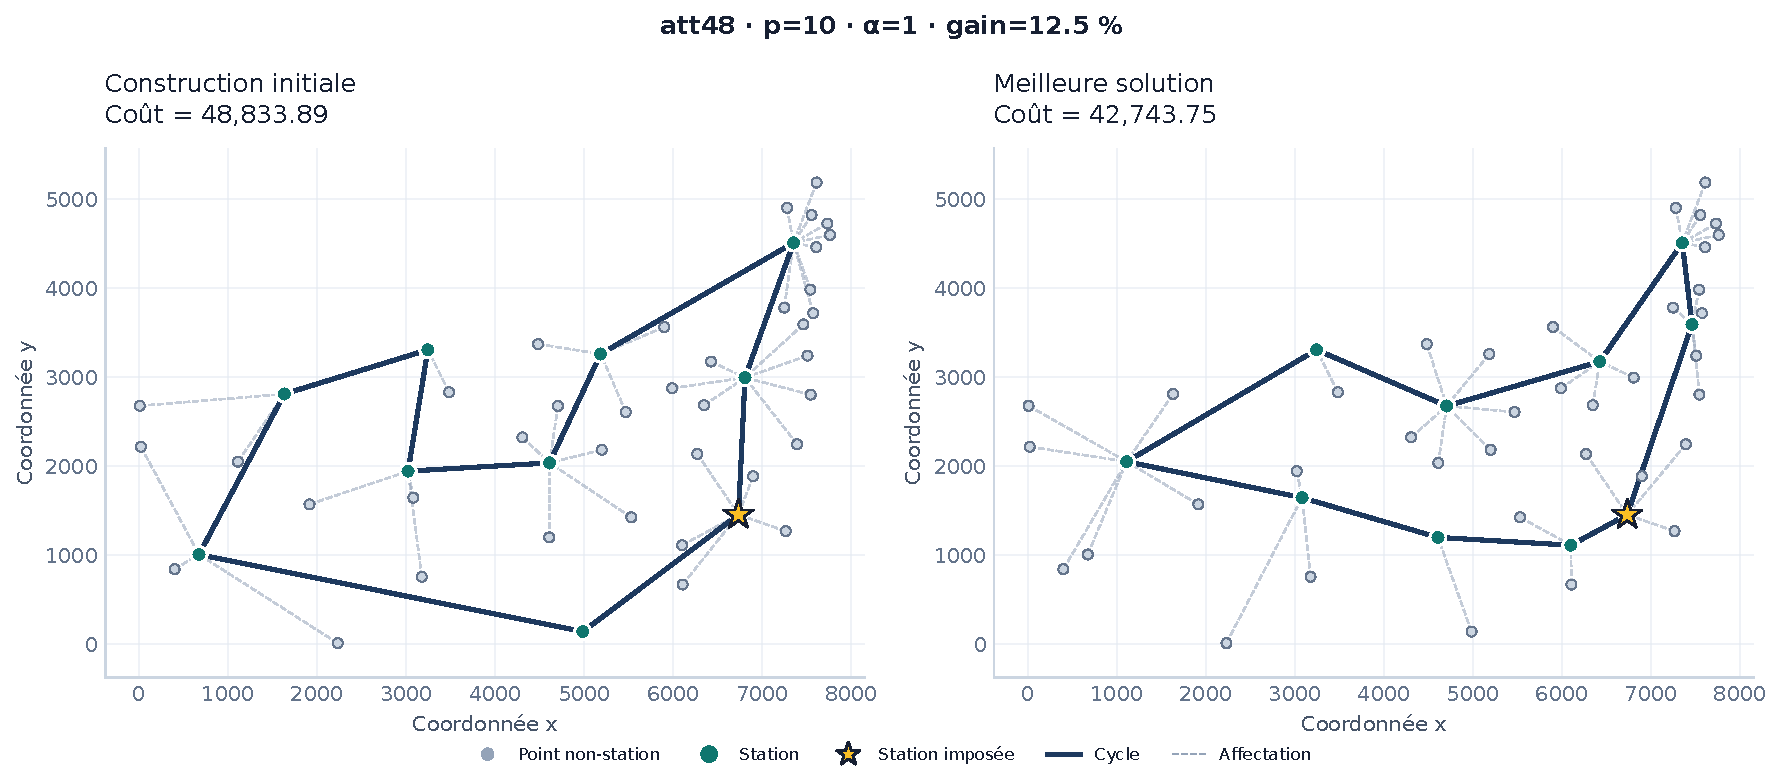
\includegraphics[width=0.99\textwidth]{figures/avant_apres_att48.pdf}
\caption{Att48, dix stations : construction puis meilleure solution tabou
de l'exécution individuelle. L'étoile distingue la station imposée.}
\label{fig:avantapres}
\sourcecalcul{exécution individuelle sauvegardée du 17 octobre 2026,
graine 0 ; 100 itérations, 15 candidats par itération, durée tabou 10.}
\end{figure}

L'anneau est mis en évidence et les traits d'affectation restent plus légers.
Une liaison d'accès plus longue n'est pas nécessairement une erreur : le
problème minimise une somme globale et ne fixe pas de distance maximale
individuelle. Une autre sélection peut donc améliorer le coût total tout en
dégradant l'accès de quelques points.

\section{D'où vient la diminution du coût ?}
Le tableau~\ref{tab:att48-decomp} décompose le résultat. Le coût total passe
de 48\,833,89 à 42\,743,75, soit un gain de 6\,090,14 unités de coordonnées
et une baisse relative de 12,47\,\%. Le README arrondit ce même pourcentage
à 12,5\,\% ; il ne s'agit pas d'un résultat différent.

\begin{table}[htbp]\centering
\begin{tabular}{lrrr}
\toprule
Composante & Construction & Meilleure tabou & Baisse relative \\
\midrule
Longueur de l'anneau & 20\,285{,}26 & 16\,477{,}53 & 18{,}77\,\% \\
Somme des accès & 28\,548{,}63 & 26\,266{,}23 & 7{,}99\,\% \\
Coût total ($\alpha=1$) & 48\,833{,}89 & 42\,743{,}75 & 12{,}47\,\% \\
\bottomrule
\end{tabular}

\caption{Décomposition du coût avant et après la recherche tabou individuelle.}
\label{tab:att48-decomp}
\sourcecalcul{coûts recalculés depuis les solutions initiale et finale sauvegardées.}
\end{table}

Dans cet exemple, les deux composantes diminuent. Ce résultat n'est pas
imposé par la recherche : seul le coût total guide le choix des mouvements.
Sur une autre instance ou avec un autre poids, une amélioration du total
pourrait augmenter l'une des composantes et réduire davantage l'autre.

La meilleure solution sélectionne les stations
$\{1,5,10,13,18,22,30,32,33,34\}$. Son cycle, lu depuis la station imposée,
est
\begin{equation*}
1\to22\to34\to5\to10\to32\to13\to33\to30\to18\to1.
\end{equation*}
L'ordre inverse représente le même cycle non orienté et le même coût.
Les affectations complètes sont conservées dans le fichier JSON de l'exécution,
ce qui permet de vérifier le résultat au-delà de l'image.

\section{Meilleure valeur et solution courante}
La trace de convergence de la figure~\ref{fig:convergence} sépare la meilleure
valeur de la valeur courante. La meilleure solution finale est atteinte
à l'itération 42, après 630 évaluations. La recherche poursuit l'exploration
jusqu'au budget de 100 itérations, sans retrouver de coût plus bas.

Le coût courant à la dernière itération est 45\,535,28, supérieur à la
meilleure valeur 42\,743,75. Ce comportement est attendu dans une recherche
qui accepte des dégradations. Exporter seulement la dernière solution aurait
perdu une partie du gain. Le programme conserve et retourne la meilleure
solution rencontrée, avec l'historique permettant de la situer dans la trajectoire.

\begin{figure}[htbp]\centering
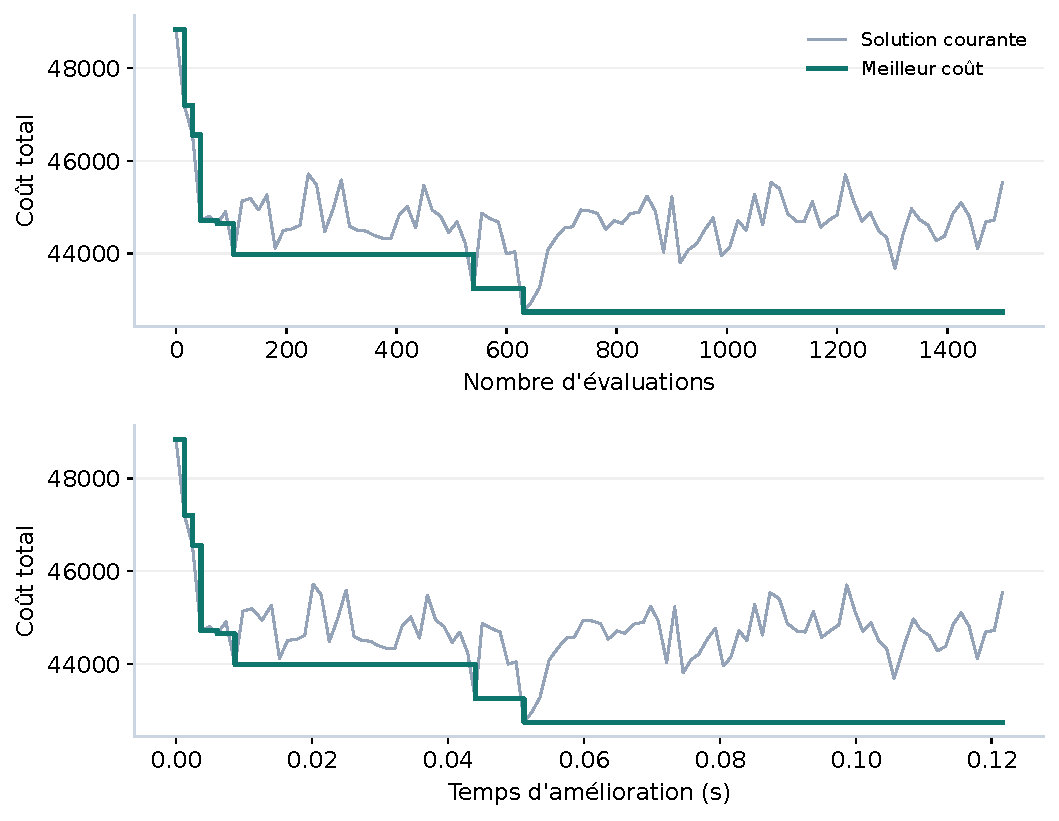
\includegraphics[width=0.98\textwidth]{figures/convergence_att48.pdf}
\caption{Coût courant et meilleure valeur : selon le nombre d'évaluations
en haut, et le temps d'amélioration en bas.}
\label{fig:convergence}
\sourcecalcul{trace sauvegardée dans \code{history.csv} pour l'exécution att48.}
\end{figure}

Le temps d'optimisation complet enregistré est d'environ 0,122 s, tandis que
l'instant d'atteinte du meilleur coût dans la trace est d'environ 0,051 s
après le début de l'amélioration. Ces durées n'incluent pas le dessin des
figures et leurs origines de mesure diffèrent légèrement, comme indiqué
dans le protocole. Leur rôle est d'éclairer cette exécution, sans promettre
la même vitesse sur toute machine.

\section{Portée de cet exemple}
Le gain avant-après est un résultat individuel. La synthèse à trois graines
de la campagne demeure la référence pour comparer les méthodes. L'exemple
ne dispose d'aucune preuve d'optimalité : il montre une amélioration
réalisable, pas la meilleure ligne possible sur les 48 points.

Il illustre aussi une limite du seul coût moyen d'accès. Ni l'accès le plus
long ni les différences entre zones ne sont pénalisés séparément. Pour un
projet de transport réel, une distance d'accès maximale, des poids de
population ou un critère d'équité pourraient modifier sensiblement le tracé.
\bilan{La figure avant-après compare une même instance et une même cardinalité.
La trace explique comment le gain est obtenu et pourquoi la meilleure
solution doit être conservée indépendamment de l'état courant.}
